\documentclass[11pt,letterpaper]{article}
\usepackage[lmargin=1in,rmargin=1in,tmargin=1in,bmargin=1in]{geometry}
\usepackage{../style/homework}
\usepackage{../style/commands}
\setbool{quotetype}{true} % True: Side; False: Under
\setbool{hideans}{false} % Student: True; Instructor: False

% -------------------
% Content
% -------------------
\begin{document}

\homework{6: Due 02/27 (28)}{The laws of probability, so true in general, so fallacious in particular.}{Edward Gibbon}

% Problem 1
\problem{10} The probabilities of several events in a finite probability space are given below:
	\[
	\begin{aligned}
	P(A)&= 0.45 & P(A \;|\; C)&= 0.10 \\
	P(B)&= 0.50 & P(B \cap C)&= 0.25 \\
	P(C)&= 0.30 & P(A \cap B)&= 0.15
	\end{aligned}
	\] 
\begin{enumerate}[(a)]
\item Find $P(A \cup B)$.
\item Find $P(B \;|\; C)$.
\item Find $P(A \cap C)$.
\item If $A$ and $C$ were independent, find $P(A \cap C)$.
\item Using (c) and (d), determine if $A$ and $C$ are independent. 
\end{enumerate} \pspace

\sol 
\begin{enumerate}[(a)]
\item We have\dots
	\[
	P(A \cup B)= P(A) + P(B) - P(A \cap B)= 0.45 + 0.50 - 0.15 \approx 0.80
	\] \pspace

\item We have\dots
	\[
	P(B \;|\; C)= \dfrac{P(B \cap C)}{P(C)}= \dfrac{0.25}{0.30} \approx 0.8333
	\] \pspace

\item We have\dots
	\[
	P(A \cap C)= P(C) P(A \;|\;C)= 0.30 \cdot 0.10 \approx 0.03
	\] \pspace

\item If $A$ and $C$ were independent, we would have\dots
	\[
	P(A \cap C)= P(A) \cdot P(C)= 0.45 \cdot 0.30 \approx 0.135
	\] \pspace

\item If $A$ and $C$ were independent, then $P(A \cap C)= P(A) \cdot P(C)$. From (c), we know that $P(A \cap C)= 0.03$. But in (d), we found $P(A) \cdot P(C)= 0.135$. But then $P(A \cap C) \neq P(A) \cdot P(C)$. Therefore, $A$ and $C$ are not independent. 
\end{enumerate}



\newpage



% Problem 2
\problem{10} Dr. Graham's 5th grade class has created a table of the number of times a school in the district has delayed or cancelled school in the last decade based on the amount of snow they received the night before. Their results are summarized below.
	\begin{table}[!ht]
	\centering
	\begin{tabular}{|l||c|c|c|c||c|} \hline
	& 0" -- 0.9" & 1" -- 2.9" & 2.9" -- 4.9" & $\geq$ 5" & Total \\ \hline \hline
	On-Time & 1200 & 800 & 350 & 5  & 2355 \\ \hline
	Delayed & 26 & 54 & 875 & 1022 & 1977 \\ \hline
	Canceled & 0 & 3 & 55 & 410 & 468 \\ \hline \hline
	Total & 1226 & 857 & 1280 & 1437 & 4800 \\ \hline
	\end{tabular}
	\end{table}

\begin{enumerate}[(a)]
\item What percentage of the time did schools cancel when it snowed?
\item What percentage of the time that it snowed did they receive 1" -- 2.9"?
\item On days when it snowed more than 5", what percentage of schools cancelled school?
\item On days when schools delayed, what percentage of those days did it snow between 0" and 0.9"?
\end{enumerate} \pspace

\sol 
\begin{enumerate}[(a)]
\item We have\dots
	\[
	P(\text{cancel and snowed})= \dfrac{468}{4800} \approx 0.0975
	\]
Therefore, schools cancelled 9.75\% of the time when it snowed. \pspace

\item We have\dots
	\[
	P(\text{receive 1" -- 2.9"})= \dfrac{857}{4800} \approx 0.1785
	\]
Therefore, the district receives 1" to 2.9" of snow 17.85\% of the time. \pspace

\item We have\dots
	\[
	P(\text{cancel} \;|\; \text{more than 5"})= \dfrac{P(\text{cancel with more than 5"})}{P(\text{more than 5"})}= \dfrac{410}{1437} \approx 0.2853
	\]
Therefore, on days when they received more than 5" of snow, schools cancelled 28.53\% of the time. \pspace

\item We have\dots
	\[
	P(\text{between 0" and 0.9"} \;|\; \text{delayed})= \dfrac{P(\text{delayed and between 0" and 0.9"})}{P(\text{delayed})}= \dfrac{26}{1977} \approx 0.0132
	\]
Therefore, on days when schools delayed, it was when there was only 0" to 0.9" of snow 1.32\% of the time. 
\end{enumerate}



\newpage



% Problem 3
\problem{10} Mr. Bobbert has a 4th grade class with 30 students. In this class, there are 18 students that like sports, 9 students that like video games, and 8 students that like both.
	\begin{enumerate}[(a)]
	\item Find the probability that a randomly selected student like sports or video games.
	\item Find the probability that a randomly selected student only likes sports. 
	\item Find the probability that a randomly selected student does not like sports nor video games.
	\item If a student enjoys video games, find the probability that they also enjoy sports. 
	\end{enumerate} \pspace

\sol We know that there are 18 students that like sports, including the 8 that like sports and video games. Therefore, $18 - 8= 10$ students like only sports. Similarly, $9 - 8$ students like only video games. Then the total number of students like that sports or video games is $10 + 8 + 1= 19$. Therefore, $30 - 19= 11$ students that like neither. Then\dots

\begin{enumerate}[(a)]
\item We have\dots
	\[
	P(\text{sports or video games})= \dfrac{10 + 8 + 1}{30}= \dfrac{19}{30} \approx 0.6333
	\] \pspace

\item We have\dots
	\[
	P(\text{only sports})= \dfrac{10}{30} \approx 0.3333
	\] \pspace

\item We have\dots
	\[
	P(\text{neither})= \dfrac{11}{30} \approx 0.3667
	\] \pspace

\item We have\dots
	\[
	P(\text{sports} \;|\; \text{video games})= \dfrac{P(\text{sports and video games})}{P(\text{video games})}= \dfrac{8}{8 + 1}= \dfrac{8}{9} \approx 0.8889
	\]
\end{enumerate} \vfill

	\[
	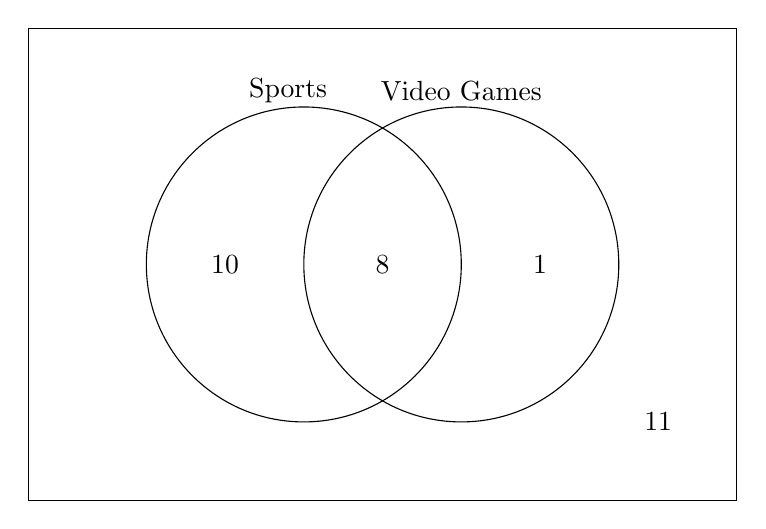
\begin{tikzpicture}
	\draw (0,0) rectangle (9,6);
	\draw (3.5,3) circle (2);
	\draw (5.5,3) circle (2);
	
	\node at (3.3,5.2) {Sports};
	\node at (5.5,5.2) {Video Games}; 
	
	\node at (2.5,3) {10};
	\node at (4.5,3) {8};
	\node at (6.5,3) {1};
	\node at (8,1) {11};
	\end{tikzpicture}
	\]



\newpage



% Problem 4
\problem{10} Ms. Streikert has a 6th grade English class. She finds that there is a 75\% chance that a student studies for an exam. If a student studies for an exam, there is an 90\% chance that they pass the exam. If a student does not study for an exam, there is a 85\% chance that they fail the exam. 
	\begin{enumerate}[(a)]
	\item Find the probability that a randomly selected student fails the exam.
	\item Find the probability that a randomly selected student studies or passes the exam.
	\item Find the probability that a randomly selected student both studies and fails the exam.
	\item If a student fails the exam, find the probability that they did not study. 
	\end{enumerate} \pspace

\sol 
\begin{enumerate}[(a)]
\item We have\dots
	\[
	P(\text{fails})= 0.0750 + 0.2125= 0.2875
	\] \pspace

\item We have\dots
	\[
	P(\text{studies or passes})= 0.6750 + 0.0750 + 0.0375= 0.7875
	\] \pspace 

\item We have\dots
	\[
	P(\text{studies and fails})= 0.0750 
	\] \pspace
  
\item We have\dots
	\[
	P(\text{not study} \;|\; \text{fails})= \dfrac{P(\text{not study and fails})}{P(\text{fails})}= \dfrac{0.2125}{0.0750 + 0.2125}= \dfrac{0.2125}{0.2875} \approx 0.73913
	\]   
\end{enumerate} \vfill

		\[
		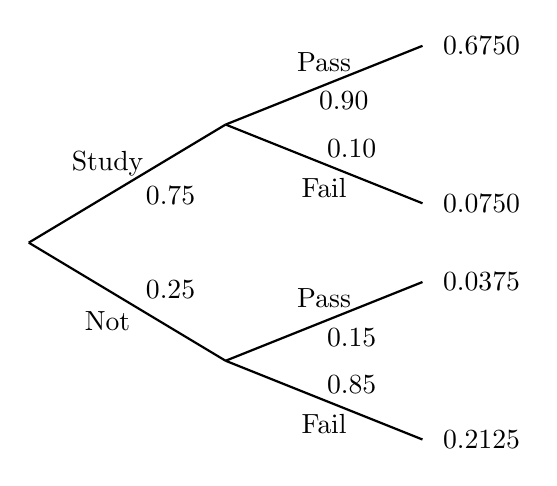
\begin{tikzpicture}[scale= 1.0]
		\def\FirstUpLabel{Study}
		\def\FirstDownLabel{Not}
		\def\SecondUpLabel{Pass}
		\def\SecondDownLabel{Fail}
		\def\Up{$0.75$}
		\def\Down{$0.25$}
		\def\UpUp{$0.90$}
		\def\UpDown{$0.10$}
		\def\DownUp{$0.15$}
		\def\DownDown{$0.85$}
		\def\first{$0.6750$}
		\def\second{$0.0750$}
		\def\third{$0.0375$}
		\def\fourth{$0.2125$}
		
		\node at (1,1) {\FirstUpLabel};	
		\node at (1,-1) {\FirstDownLabel};	
		\node at (1.8,0.6) {\Up};
		\node at (1.8,-0.6) {\Down};
		\draw[thick] (0,0) -- (2.5,1.5);
		\draw[thick] (0,0) -- (2.5,-1.5);
		
		\node at (3.75,2.3) {\SecondUpLabel};
		\node at (3.75,0.7) {\SecondDownLabel};
		\node at (4,1.8) {\UpUp};
		\node at (4.1,1.2) {\UpDown};
		\node at (5.75,2.5) {\first};
		\node at (5.75,0.5) {\second};
		\draw[thick] (2.5,1.5) -- (5,2.5);
		\draw[thick] (2.5,1.5) -- (5,0.5);

		\node at (3.75,-0.7) {\SecondUpLabel};
		\node at (3.75,-2.3) {\SecondDownLabel};
		\node at (4.1,-1.2) {\DownUp};
		\node at (4.1,-1.8) {\DownDown};
		\node at (5.75,-0.5) {\third};	
		\node at (5.75,-2.5) {\fourth};	
		\draw[thick] (2.5,-1.5) -- (5,-0.5);
		\draw[thick] (2.5,-1.5) -- (5,-2.5);
		\end{tikzpicture}
		\]


\end{document}